%%\chapter*[Introdução]{Introdução}
%%\addcontentsline{toc}{chapter}{Introdução}

%%Este documento apresenta considerações gerais e preliminares relacionadas 
%%à redação de relatórios de Projeto de Graduação da Faculdade UnB Gama 
%%(FGA). São abordados os diferentes aspectos sobre a estrutura do trabalho, 
%%uso de programas de auxilio a edição, tiragem de cópias, encadernação, etc.

%%Este template é uma adaptação do ABNTeX2\footnote{\url{https://github.com/abntex/abntex2/}}.


\chapter[INTRODUÇÃO]{INTRODUÇÃO}
\section{Contexto e Justificativa}

O Instituto de Aviação Varsóvia (ILOT, do polonês \textit{Instytut Lotnictwa}) e a Universidade de Brasília (UNB) decidiram firmar uma cooperação tecnológica, em novembro de 2014. Entre várias oportunidades, essa cooperação possibilita estágios para alunos de graduação em Engenharia Aeroespacial no ILOT. Uma nova proposta está sendo discutida entre os pesquisadores das duas instituições, visando a criação de uma missão 3U CubeSat.

Essa missão será destinada à validação de conceitos e teste de componentes, enquadrando-se como demonstrador tecnológico. Os objetivos iniciais, levantados pelos pesquisadores, são: uso de câmeras para monitoramento das calotas polares, com o intuito de estudar os efeitos da poluição; uso de um \textit{Pulsed Plasma Thruster} (PPT) para estudo de controle orbital;  uso de um acelerômetro para mapeamento do campo gravitacional terrestre.

Um projeto desse porte abrirá várias oportunidades de pesquisa na área de subsistemas satelitais, sensoriamento remoto, controle orbital, entre outros. Alguns estudos já estão sendo realizados, com o intuito de oferecer soluções para essa futura missão. O presente trabalho faz parte dessa série de pesquisas e tem o intuito de realizar a construção de um computador de bordo (OBC, do inglês \textit{On-Board Computer}) para CubeSats.



\section{Objetivos}

Este trabalho tem como objetivo principal o desenvolvimento de um OBC para o controle e gerenciamento do CubeSat UNB-ILOT.  Os objetivos específicos são:

\begin{itemize}
	
	\item Controle de uma Câmera CMOS (do inglês \textit{Complementary Metal-Oxide-Semiconductor});
	\item Controle de um PPT;
	\item Garantir um subsistema com um alto nível de confiança, mesmo não utilizando dispositivos resistentes à radiação;
	\item Divulgação da pesquisa na plataforma GitHub.
	
\end{itemize}


\section{Metodologia}
\label{metodo}
Inicialmente foi realizada uma pesquisa bibliográfica para reunir informações que dariam base ao projeto. Nessa fase foi analisado: ambiente espacial; pequenos satélite, mais especificamente os CubeSats; OBCs (\textit{hardware} e \textit{software}) de missões passadas e disponíveis à venda.

Após a pesquisa bibliográfica, foi realizado o levantamento dos requisitos da missão com o intuito de definir as funcionalidades e delimitar o escopo da pesquisa.

Logo em seguida, foi feito o projeto preliminar do sistema. Para a parte de \textit{hardware}, foi escolhido: o microcontrolador, sensores, memória; entre outros. Já para o \textit{software}, escolheu-se: a arquitetura, linguagem de programação, sistema operacional; etc. Vale ressaltar que optou-se por uma concepção conjunta (do inglês \textit{Co-Design}) do \textit{hardware} e \textit{software}, em que o desenvolvimento de ambos acontece simultaneamente.

Em paralelo ao estudo preliminar, foram realizados testes em \textit{protoboard}, visando a validação de alguns subsistemas separadamente. Esses testes foram de extrema importância, pois, aumentaram as chances do sistema funcionar nas fases de prototipagem final. Nessa fase, os códigos para cada subsistema foram testados e, em seguida, unidos em um único código.

\hl{*********}
Por fim, após a validação do sistema em \textit{protoboard}, será feito o  projeto final do sistema. Para a parte de \textit{hardware}, serão entregues os esquemáticos, \textit{layout} da PCB (do inglês \textit{Printed Circuit Board}), BOM (do inglês \textit{Bill of Materials}) e simulações de circuitos analógicos. Para a parte de \textit{software}, será entregue a arquitetura do sistema, diagrama UML (do inglês \textit{Unified Modeling Language}) e fluxograma das rotinas.
\hl{*********}

A Figura \ref{fig01} mostra o fluxograma para o projeto do OBC.
\begin{comment}
O TCC2 visará a criação da placa de circuito impresso, prototipagem, teste da placa, alterações finais e, por fim, a entrega do produto final. 

\end{comment}


\begin{figure}[!h]
	\centerfloat
	\centering
	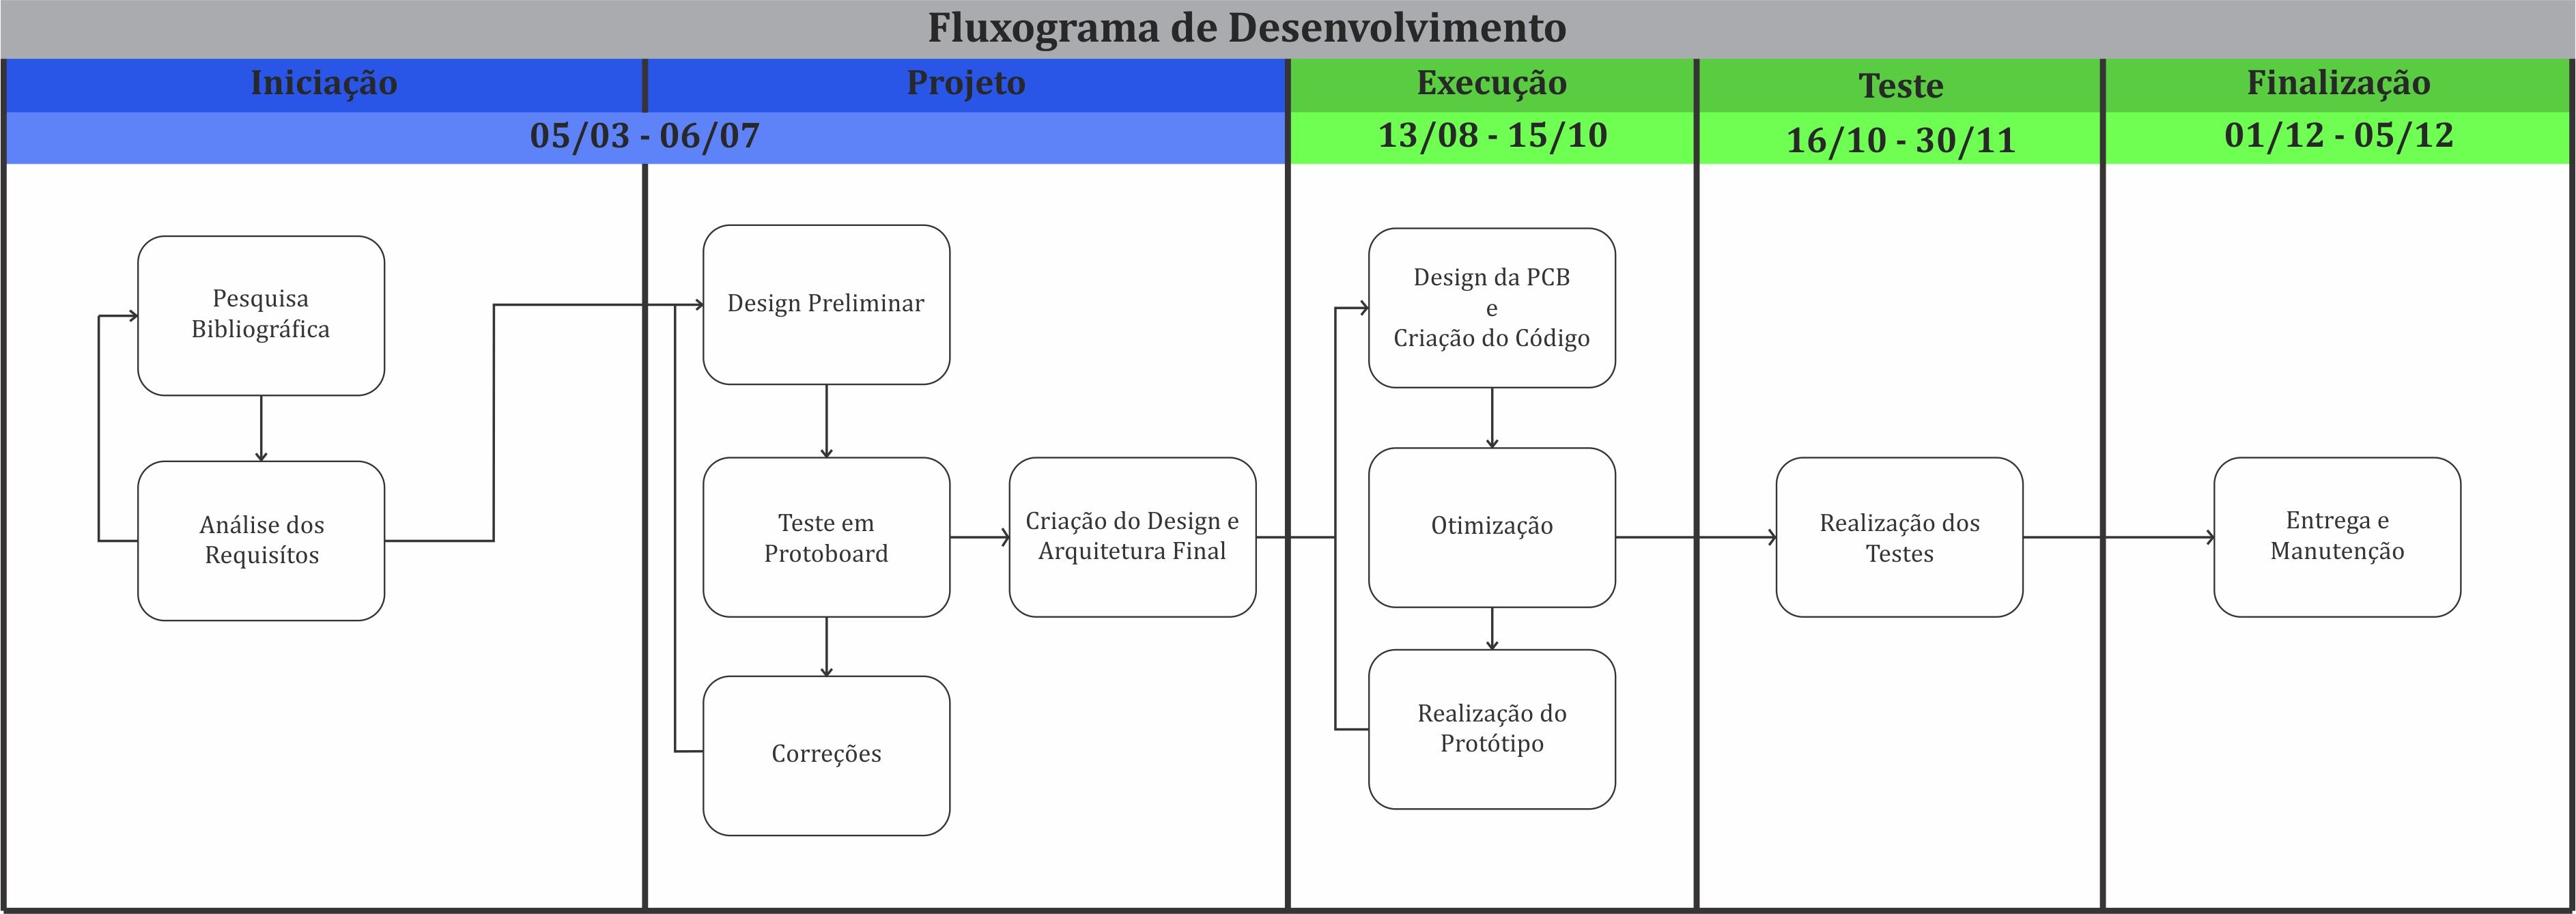
\includegraphics[keepaspectratio=true,scale=0.54	]{figuras/cronograma_2.jpg}
	\caption{Cronograma do Trabalho de Pesquisa.}
	\label{fig01}
\end{figure}

